\documentclass[11pt,a4paper]{article}
\usepackage[margin=2.3cm]{geometry}
\usepackage[T1]{fontenc}
\usepackage{lmodern}
\usepackage{amsmath,amssymb,amsthm}
\usepackage{booktabs,array,tabularx}
\usepackage{graphicx}
\usepackage{xcolor}
\usepackage{enumitem}
\usepackage[hidelinks]{hyperref}
\usepackage{microtype}
\setlist{itemsep=2pt,topsep=4pt}
\definecolor{flag}{HTML}{B4380F}
\newcommand{\assume}{\textcolor{flag}{\textsuperscript{[A]}}}
\newtheorem{proposition}{Proposition}
\newcommand{\E}{\mathbb{E}}
\newcommand{\Var}{\operatorname{Var}}
\renewcommand{\arraystretch}{1.15}

\title{\textbf{Returning 60 Marked Quizzes}\\[4pt]
\large A stochastic simulation of five hand-back methods in two lecture rooms\\[2pt]
\normalsize Technical report: model, mathematics, assumptions, data and results}
\author{Muhammad B.\ Arif\\ \small University College Dublin}
\date{November 2026}

\begin{document}
\maketitle

\begin{abstract}
\noindent
A lecturer has 60 marked quizzes to return to the roughly 50 students present in a class, without reading names aloud and without losing teaching time.
We built an agent-based, discrete-time simulation of two real lecture rooms and compared five methods: one stack passed along the class, two stacks started at opposite ends, one stack per table, calling names, and a pile on the lecturer's desk after class.
Movement uses a grid (cellular-automaton) pedestrian model, and finding one's own sheet in a stack is modelled as a serial self-terminating search whose probabilities follow directly from a uniformly random shuffle.
Each method was run in 500 randomly generated classes per room, with common random numbers so that every method faces the same classes, giving 5{,}000 simulated classes in total.
Passing a single stack costs the lecturer only 2--8\,s of teaching but takes about 14 minutes; one stack per table is fastest during class (5.2--6.0\,min) but costs 38--87\,s of teaching, keeps 8--10 students busy at once and makes students get up 26--31 times; the after-class pile takes about 5.5 minutes of everyone's time after class.
All code, parameters and raw results are public, and the code is checked against closed-form probability results.
Parameters marked \assume{} are assumptions, not measurements.
\end{abstract}

\tableofcontents
\newpage

%=====================================================================
\section{The question}

\paragraph{Problem.} About 60 quizzes, about 50 students present, a 50-minute class. Three constraints:
\begin{enumerate}
  \item \textbf{Time:} the return should not eat into teaching.
  \item \textbf{Accuracy:} every student present gets their own quiz.
  \item \textbf{Privacy:} quizzes of absent students should come back to the lecturer rather than be left lying around (a GDPR concern), and as few people as possible should see other students' sheets.
\end{enumerate}

\paragraph{Why simulate?} The methods differ in ways that are hard to judge by intuition: where people walk, how often they wait, and especially how long it takes to find one sheet in a stack.
The idea follows simulation studies of aircraft boarding, which compare boarding orders using the same kind of agent-based model \cite{steffen2008}.

\paragraph{Methods compared.}
\begin{enumerate}[label=\textbf{\arabic*.}]
  \item \textbf{One stack, passed along:} the lecturer hands the whole stack to one student at the start of class and keeps teaching.
  \item \textbf{Two stacks, one from each end:} the stack is split at random in two; each half starts at one end.
  \item \textbf{One stack per table:} the lecturer places one small stack on every occupied table (G24: each half-row).
  \item \textbf{Calling names:} the lecturer reads each name and walks the quiz to the student.
  \item \textbf{Pile on the lecturer's desk, after class:} everyone collects their own quiz on the way out.
\end{enumerate}

%=====================================================================
\section{Overview of the model}

The model is an \emph{agent-based, discrete-time stochastic simulation}.
Each student and the lecturer is an agent with a position, a walking speed and (for students) a searching speed.
Time advances in steps of $\Delta t = 0.1$\,s. At every step each agent updates its task (searching, handing over, walking, queueing) and moves on the grid.
A run ends when every present student has their quiz or has definitively failed to get it, all stacks have finished, and the leftovers are with the lecturer.

The model has three layers:
\begin{enumerate}
  \item \textbf{Space and movement} (Section~\ref{sec:space}): rooms on a grid; shortest-path walking; a floor-field crowd model for the pile.
  \item \textbf{Search} (Section~\ref{sec:search}): the probability model for finding one's own sheet, derived from first principles.
  \item \textbf{Method rules} (Section~\ref{sec:methods}): who holds which stack, where it goes next, and what the lecturer does.
\end{enumerate}
Section~\ref{sec:experiment} describes the Monte Carlo experiment, Section~\ref{sec:verification} how the code was verified, and Section~\ref{sec:results} the results.

%=====================================================================
\section{Space and movement}\label{sec:space}

\subsection{The grid}
The floor is divided into square cells of $0.4\,\text{m}\times 0.4\,\text{m}$, and a cell holds at most one person.
This is the standard cell size in cellular-automaton (CA) pedestrian models \cite{burstedde2001,kirchner2002}: it gives a maximum density of $1/0.16 = 6.25$ persons/m$^2$, close to the observed jam density of about 5.4 persons/m$^2$ \cite{weidmann1993}.
Tables, benches and the desk are blocked cells. Seats are cells next to the furniture.

\subsection{Room geometry: estimated, not measured}
\textbf{Important:} the room dimensions are estimates. The layouts (number and arrangement of tables and benches, doors, desk) come from the lecturer's sketches; the sizes in metres were chosen from typical furniture sizes.
They are stored in plain text files (\texttt{config/rooms/*.yaml}) and will be replaced by measured values.

\begin{table}[htbp]\centering\small
\begin{tabularx}{\textwidth}{lXX}
\toprule
 & \textbf{E1.17 (round tables)} & \textbf{G24 (benches)} \\
\midrule
Room size\assume & $16.0 \times 10.0$\,m ($40\times25$ cells) & $18.0\times 11.6$\,m ($45 \times 29$ cells) \\
Furniture\assume & 8 round tables in 2 rows of 4, radius 0.8\,m, centres 3.6\,m apart & 5 rows $\times$ 2 banks of benches, 0.8\,m deep, row pitch 1.6\,m, 2.0\,m centre aisle \\
Seats & 8 per table at 1.2\,m from the centre: \textbf{64 seats} & left bank 7, right bank 11 per row, 0.8\,m apart: \textbf{90 seats} \\
Occupancy (50 students) & 78\,\% & 56\,\% \\
Doors & two, front corners & one, front left wall \\
Lecturer & desk front-centre; teaching spot to the left of it & desk front-centre; teaching spot front-left \\
Other & -- & the 0.4\,m gaps behind bench seats are ``narrow'': students can squeeze through, the lecturer cannot \\
\bottomrule
\end{tabularx}
\caption{Room geometry used. Values marked \assume{} are estimates from sketches.}
\end{table}

\begin{figure}[htbp]\centering
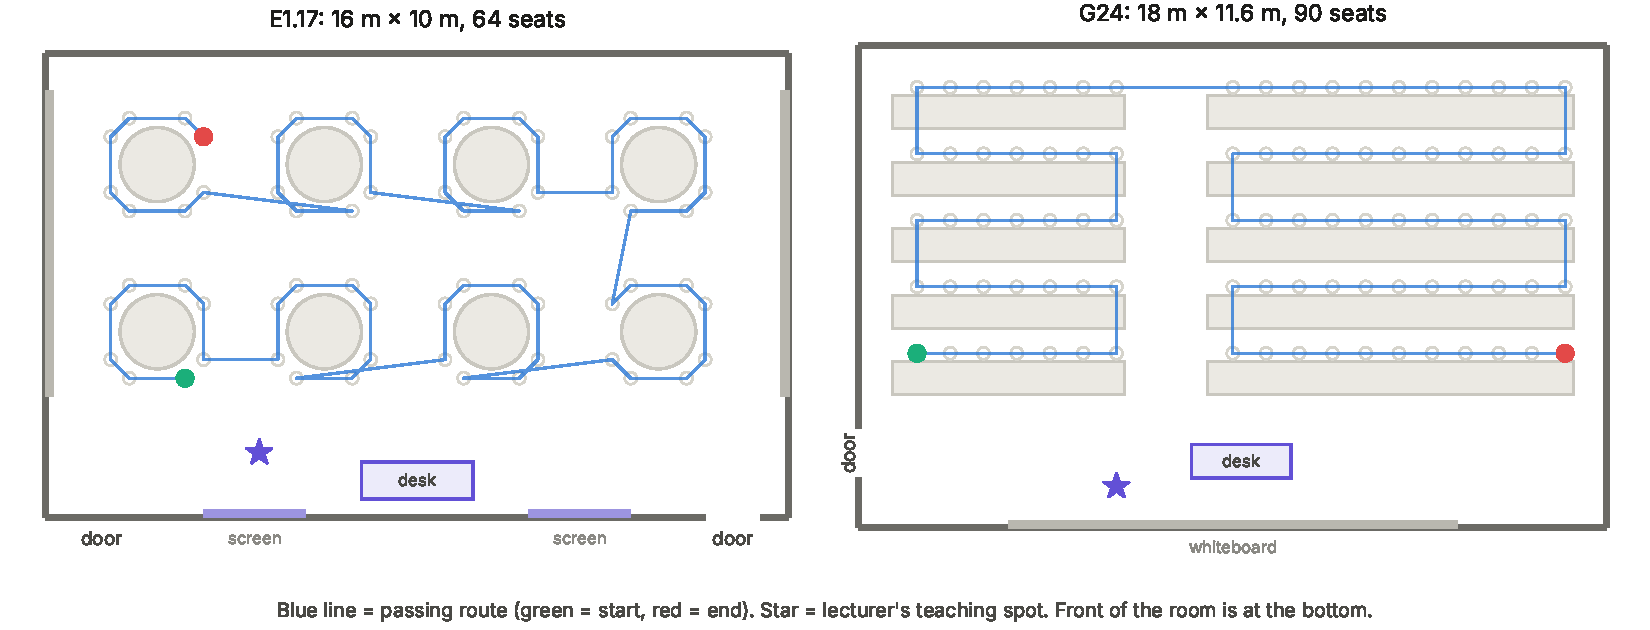
\includegraphics[width=\textwidth]{fig/rooms.pdf}
\caption{The two rooms as modelled, with the fixed passing route used by the stack methods (Section~\ref{sec:route}).}
\end{figure}

\paragraph{How much the estimated geometry matters.}
In the stack methods most of the time is spent searching and handing over, which does not depend on room size; passing along a row depends only on seat spacing.
Walking matters more for calling names (the lecturer walks to every student), for one stack per table (table-to-table walks and the lecturer placing stacks) and for the pile (walking to and from the desk).
These are the results most likely to shift when measured dimensions are used.

\subsection{Walking speed}
Each person's free walking speed is drawn once per run:
\[
v_0 \sim \mathcal{N}(1.34,\ 0.26^2)\ \text{m/s, clipped to } [0.7,\,2.0],\qquad v = 0.8\,v_0 .
\]
The normal distribution and its parameters are Weidmann's synthesis of measured pedestrian speeds \cite{weidmann1993}.
The factor 0.8\assume{} represents walking between furniture rather than on an open walkway; the mean effective speed is therefore about 1.07\,m/s.

\subsection{Walking to a target}
An agent going somewhere (to the next student, to the desk, back to their seat) follows a shortest path on the 8-connected grid: orthogonal steps cost 0.4\,m and diagonal steps $0.4\sqrt2 \approx 0.57$\,m.
Paths are computed with Dijkstra's algorithm \cite{dijkstra1959}. Diagonal steps may not cut the corner of furniture, and seated students are obstacles.
Movement is continuous in time: an agent accumulates distance $v\,\Delta t$ each step and enters the next cell once the accumulated distance reaches that step's length.
Conflicts are resolved as follows:
\begin{itemize}
  \item If the next cell is occupied, the agent waits. After 2\,s of waiting it recomputes its path treating all occupied cells as obstacles.
  \item If someone has settled on the agent's goal cell (other than its own seat), the goal moves to the nearest free neighbouring cell.
  \item Two agents heading into each other's cells step past each other (swap), which prevents head-on deadlock in narrow gaps.
\end{itemize}

\subsection{Crowd movement (pile method only)}
For the after-class pile, many people move at once towards one point, so we use the floor-field cellular automaton of Burstedde et al.\ \cite{burstedde2001} and Kirchner and Schadschneider \cite{kirchner2002}.
\begin{itemize}
  \item \textbf{Floor fields.} A \emph{static floor field} $S(x)$ gives the walking distance from every cell $x$ to the target (the spots at the desk, or the doors), computed once by Dijkstra's algorithm.
  \item \textbf{Moving.} At each step, people are updated in random order (\emph{random sequential update}). Each person moves to the free neighbouring cell with the lowest $S$, provided they have accumulated enough distance; ties are broken at random.
  \item \textbf{Leaving through the queue.} Someone leaving may swap places with someone still queueing, with probability 0.3 per step, so the two flows can pass each other.
  \item \textbf{Getting unstuck.} A blocked person shuffles sideways to an equally good free cell with probability 0.2 per step.
  \item \textbf{The lecturer} sits behind the desk; that cell is excluded from the floor fields.
\end{itemize}
This is a deterministic-gradient simplification of the original model: it has no dynamic field and no sensitivity parameter, because the goal here is queue formation at a single point, not lane formation.

%=====================================================================
\section{Finding your own quiz: the probability model}\label{sec:search}

This is the core of the model: for the stack methods it determines most of the total time.

\subsection{Position of your sheet in a shuffled stack}
A stack of $n$ sheets is a uniformly random permutation: every one of the $n!$ orders is equally likely. A student flicks from the top until they reach their own sheet. Let $K$ be its position.

\begin{proposition}[Uniform position]
If the stack is uniformly shuffled and contains your sheet, then $P(K=k) = 1/n$ for $k = 1,\dots,n$.
\end{proposition}
\begin{proof}
By symmetry, the number of permutations with your sheet in position $k$ is $(n-1)!$ for every $k$, so the probability is $(n-1)!/n! = 1/n$.
Sequentially: the top sheet is yours with probability $1/n$; given it is not, the next is yours with probability $1/(n-1)$; and so on. Hence
\[
P(K=k) = \frac{n-1}{n}\cdot\frac{n-2}{n-1}\cdots\frac{n-k+1}{n-k+2}\cdot\frac{1}{n-k+1} = \frac1n .\qedhere
\]
\end{proof}
Therefore
\[
\E[K] = \frac{n+1}{2},\qquad \Var[K] = \frac{n^2-1}{12},\qquad P(K\le k) = \frac{k}{n}.
\]
For $n=60$: $\E[K]=30.5$, the standard deviation is $17.3$, and there is a 50\,\% chance of finding your sheet within the first 30.
The conditional chance of ``the next one is mine'' grows from $1/60$ to $1$, but the unconditional chance of any specific position is always $1/60$.

\begin{proposition}[The stack stays shuffled as it shrinks]
If one sheet is removed from a uniformly random permutation, the remaining $n-1$ sheets are in uniformly random order.
\end{proposition}
\begin{proof}
Each order of the remaining sheets arises from exactly $n$ orders of the full stack (one for each position of the removed sheet), so all $(n-1)!$ orders are equally likely.
\end{proof}
So when the stack passes from student to student it remains uniformly shuffled, and the next student faces the same law with $n$ reduced by one.
In the code the stack \emph{is} a list in random order and $K$ is read off it; uniformity is not imposed by a formula but emerges from the shuffle, and is checked empirically in Section~\ref{sec:verification}.

\subsection{From sheets to seconds}
Search time is modelled as
\[
T = a + b\,C,
\]
where $C$ is the number of sheets checked ($C=K$ if nothing goes wrong). This is the linear set-size function of \emph{serial self-terminating search} from visual-search research \cite{treisman1980,wolfe1998}.
\begin{itemize}
  \item $a = 3.0$\,s\assume: pick up the stack and start.
  \item $b$: seconds per sheet (read a name, flick). Each student has their own $b$, drawn once per run from a log-normal distribution with mean $0.6$\,s\assume{} and coefficient of variation $0.3$\assume.
\end{itemize}
Reading a single short word takes roughly 0.25\,s \cite{brysbaert2019}; flipping a paper sheet adds motor time, and 0.6\,s was agreed as plausible with the lecturer. The log-normal reflects the right skew of human response times \cite{luce1986}: most people are near typical speed, and a few are much slower. Its parameters are
\[
\sigma = \sqrt{\ln(1+0.3^2)} = 0.2936,\qquad \mu = \ln 0.6 - \sigma^2/2 = -0.5539 .
\]
Because a student's speed $b$ is independent of where their sheet lies, $\E[T] = a + \E[b]\,\E[C]$. For a full stack of 60: $\E[T] = 3 + 0.6\times30.5 = 21.3$\,s, with range $3.6$--$39$\,s at $b=0.6$.

\subsection{Missing your own sheet}
When a student reaches their own sheet they flick past it with probability $q = 0.02$\assume. There are only misses (false negatives), never false positives: nobody takes someone else's quiz.
\begin{itemize}
  \item After a miss the student checks the rest of the stack ($n$ sheets in total for that pass).
  \item If the student knows their sheet must be in this stack (``certain''; Section~\ref{sec:certain}), they go through once more, up to two passes. The order is unchanged, so their sheet is again at position $K$.
\end{itemize}
With two passes, the probability of ending without the quiz is $q^2 = 0.0004$, and
\[
\E[C] = (1-q)\,\E[K] + q(1-q)\,\bigl(n+\E[K]\bigr) + q^2\cdot 2n,
\]
which is $31.71$ for $n=60$.

\subsection{Several stacks: your sheet may not be in the one you get}\label{sec:multi}
Suppose $R$ sheets are split at random into $s$ stacks of $m = R/s$, and a student sees them in some order.
Stack $j$ contains the student's sheet, given the first $j-1$ did not, with probability
\[
\frac{m}{R-(j-1)m} = \frac{1}{s-j+1},
\]
so for 4 stacks of 15 the probabilities are $25\,\%, 33\,\%, 50\,\%, 100\,\%$. Unconditionally, the index $J$ of the right stack is uniform on $\{1,\dots,s\}$, so $\E[J] = (s+1)/2$.
For each wrong stack the student checks all $m$ sheets, and in the right one $(m+1)/2$ on average:
\[
\E[C] = m\,\frac{s-1}{2} + \frac{m+1}{2} = \frac{sm+1}{2} = \frac{R+1}{2}.
\]
\textbf{Splitting the stack does not reduce the expected number of sheets each student reads.} It is exactly the same as one big stack. Splitting helps only because several students search in parallel, and it costs waiting time for the right stack to arrive.

\subsection{When is a student ``certain''?}\label{sec:certain}
A student who has a stack in hand is certain their sheet is in it when every other stack is either already seen by them or empty, i.e.\ this is the last stack they have not seen.
Only then does a miss lead to a second pass. A miss in a non-final stack therefore means the student never gets their quiz. This is why the multi-stack methods have slightly more unclaimed quizzes (about $q\times(1-1/s)$ per student).

\subsection{Privacy exposure}
For each search we record the number of distinct \emph{other} students' sheets the student looked at:
$K-1$ if found on the first pass, $n-1$ if after a miss, and $n$ if their sheet was not in the stack.
The reported metric is the total per run divided by the 50 students.

%=====================================================================
\section{Method rules}\label{sec:methods}

\subsection{Common rules for the stack methods (1--3)}\label{sec:route}
\begin{itemize}
  \item \textbf{Fixed passing route.} Students are told to pass to the person next to them, so a stack follows a fixed route through the seats.
  \begin{itemize}
    \item \textbf{G24:} a snake. The left bank runs front to back, along each row and then into the row behind, ending at the aisle. The stack crosses the aisle once, at the back, and the right bank runs back to front.
    \item \textbf{E1.17:} round each table. The tables are visited in a snake (front row left to right, back row right to left). Each table starts at the seat nearest the previous table, and the direction round it is chosen to end nearest the next table.
  \end{itemize}
  \item \textbf{Who gets it next.} The next person on the route who has not had this stack. Someone who already has their quiz just passes it on (one hand-over).
  \item \textbf{Hand-overs.} Each takes 2.0\,s\assume.
  \begin{itemize}
    \item On the same bench or table it is always seated; the stack slides past empty seats at $+0.6$\,s per metre beyond 2.5\,m\assume.
    \item To another row or table it is seated if the seats are within 2.5\,m\assume{} (both students lean across). Otherwise the holder walks it over and walks back.
  \end{itemize}
  \item \textbf{One stack at a time.} A student holds one stack at a time; others wait in front of them in arrival order.
  \item \textbf{End of a stack.} When nobody further along still needs it, the leftovers are passed forward, seated where possible, to ever closer students until they reach the student sitting nearest the desk (the \emph{collector}). The collector keeps all leftover stacks until every stack has finished, then takes them up in one trip (1.0\,s to put them down). A stack that runs out of sheets simply stops.
  \item \textbf{Lecturer.} Their time spent walking out, handing over and walking back is \emph{teaching time lost}.
\end{itemize}

\subsection{The five methods}
\begin{description}[style=nextline]
  \item[1. One stack] The full shuffled stack goes to the first student on the route.
  \item[2. Two stacks] The stack is split at random 30 + 30. One half starts at each end of the route, travelling in opposite directions. Each must reach everyone still looking, so the two cross.
  \item[3. One stack per table] The stack is split at random into one stack per occupied table (E1.17: up to 8 tables; G24: up to 10 half-rows). The lecturer walks the route placing them. Each stack goes round its table, then to the next table on the route, where it is handed to whoever is nearest and goes round that table from them. This continues cyclically until nobody still needs it.
  \item[4. Calling names] For each sheet in stack order:
  \begin{itemize}
    \item The lecturer reads the name: 2.0\,s\assume, repeated with probability 0.3\assume{} (up to twice), because the names are hard for this lecturer to pronounce.
    \item An absent student costs 4.0\,s\assume{} of silence, and the sheet stays with the lecturer. A present student fails to recognise their name with probability 0.02\assume{} and is treated the same way.
    \item Otherwise a hand goes up after 1.5\,s\assume{} and the lecturer walks over, handing it directly from within 1.0\,m.
    \item In G24 the lecturer cannot enter the gaps behind the benches. For a student deep in a row, the lecturer hands the quiz to the nearest reachable point and it is passed along the bench, taking $\max\{1,\operatorname{round}((d-0.6)/0.8)\}$ passes of 1.5\,s\assume{} each, while the lecturer moves on.
    \item All of this time is teaching time lost.
  \end{itemize}
  \item[5. Pile on the desk, after class] Students pack up for $U(0,20)$\,s\assume, then walk to the desk with the crowd model.
  \begin{itemize}
    \item Only the 8 spots directly along the front of the desk give access, and at most $c=4$\assume{} people handle the pile at once.
    \item When someone gets a turn, the current pile, in its shuffled order, is split into $\min(4,R)$ chunks. They search the chunks in random order (the multi-stack model above), waiting 3.0\,s\assume{} for each further chunk, and are certain on the last chunk.
    \item Everyone else queues. Patience is effectively unlimited: the lecturer reports that every student present always collects theirs, and only the absentees' quizzes are left over.
    \item People leave by any door. One approximation: removals by other searchers during someone's search are not reflected in their chunks until their next search.
  \end{itemize}
\end{description}

%=====================================================================
\section{The Monte Carlo experiment}\label{sec:experiment}

\subsection{What is random in one simulated class}
Run $r$ uses seed $r\in\{0,\dots,499\}$. From a generator seeded with $r$ (NumPy's PCG64 \cite{oneill2014}) the following are drawn, \emph{in this order}:
\begin{enumerate}
  \item which 50 of the room's seats are occupied (uniform, without replacement);
  \item the shuffle of the 60 quizzes (uniform random permutation; quizzes 0--49 belong to the students present, 50--59 to the absentees);
  \item walking speeds of the 50 students and the lecturer;
  \item each student's search speed $b$.
\end{enumerate}
Everything that happens during the method (misses, repeats, chunk orders, crowd updates) uses a second generator seeded with $(r, 7)$.

\subsection{Common random numbers}
Because steps 1--4 depend only on the seed, \textbf{every method faces the identical class} for a given seed: same seating, same shuffle, same people. This is the variance-reduction technique of \emph{common random numbers} \cite{law2015}. Differences between methods therefore reflect the method, not luck, and paired comparisons are possible (Table~\ref{tab:paired}).

\subsection{Sample size and statistics}
\begin{itemize}
  \item \textbf{Size:} 500 classes $\times$ 5 methods $\times$ 2 rooms = 5{,}000 simulated classes, about 15 minutes on two CPU cores.
  \item \textbf{Reported per method and room:}
  \begin{itemize}
    \item the \textbf{median} finish time (a typical class), with a 95\,\% bootstrap confidence interval (4{,}000 resamples, percentile method \cite{efron1993});
    \item the \textbf{10th--90th percentile range}: 8 in 10 classes fall inside it.
  \end{itemize}
  \item \textbf{Why the median:} finish times are right-skewed, especially for calling names, so the median is the more representative ``typical class''.
  \item \textbf{Precision:} the standard error of the median is roughly $1.25\,\sigma/\sqrt{500} \approx 3$--$7$\,s here, small compared with the differences between methods.
\end{itemize}

\subsection{Metrics}
\begin{description}
  \item[Finish time] From the start of the method until every present student has their quiz or has failed definitively, every stack has finished, and the leftovers are with the lecturer. For the pile this is time after class.
  \item[Unclaimed] Present students who end without their quiz.
  \item[Teaching time lost] The lecturer's time spent on the return during class.
  \item[Distraction] Student-minutes spent searching, handing over or walking during class.
  \item[Times a student gets up] Number of walks a student makes to carry a stack to another row or table, or the leftovers to the desk (during class). For the pile, everyone gets up.
  \item[Most busy at once] The peak number of students simultaneously occupied with the return (searching, handing over, walking).
  \item[Privacy exposure] Other students' sheets seen per student.
\end{description}

%=====================================================================
\section{Verification}\label{sec:verification}

\subsection{Code against the mathematics}
\texttt{tests/test\_search\_math.py} runs the actual search function on 200{,}000 freshly shuffled stacks per check and compares the results with Section~\ref{sec:search}. A check fails if the difference exceeds four standard errors.

\begin{table}[htbp]\centering\small
\begin{tabular}{lrrr}
\toprule
Check & Formula & Simulated & $\pm$1 SE \\
\midrule
Stack of 60: $P(K=1)$ & 0.0167 & 0.0163 & 0.0003 \\
Stack of 60: $P(K\le 10)$ & 0.1667 & 0.1644 & 0.0008 \\
Stack of 60: $P(K\le 30)$ & 0.5000 & 0.4989 & 0.0011 \\
Stack of 60: $\E[K]$ & 30.50 & 30.57 & 0.04 \\
Stack of 60: $\E[T]$ (s) & 21.30 & 21.33 & 0.03 \\
$q=2\%$: $P(\text{not found after 2 passes}) = q^2$ & 0.0004 & 0.0004 & 0.00005 \\
$q=2\%$: $\E[C]$ & 31.71 & 31.63 & 0.04 \\
4 stacks of 15: $P(J=1)$ & 0.250 & 0.250 & 0.001 \\
4 stacks of 15: $P(J=2)$ & 0.250 & 0.250 & 0.001 \\
4 stacks of 15: $\E[J]$ & 2.50 & 2.50 & 0.003 \\
4 stacks of 15: $\E[C]$ & 30.50 & 30.52 & 0.04 \\
\bottomrule
\end{tabular}
\caption{Formula versus simulation. The goodness-of-fit of all 60 positions to the uniform law gives $\chi^2 = 63.2$ on 59 degrees of freedom (critical value 99.6 at $p=0.001$). The largest deviation ($P(K\le10)$, 2.9 SE) is within the expected spread for eleven simultaneous checks.}
\end{table}

\begin{figure}[htbp]\centering
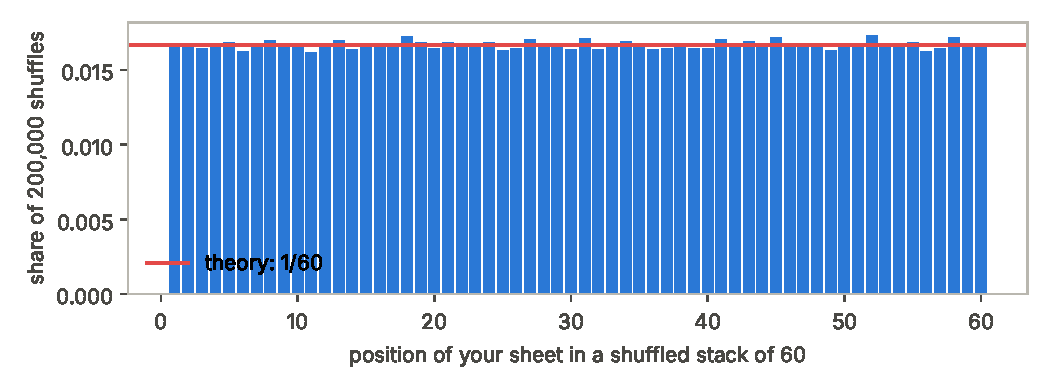
\includegraphics[width=0.8\textwidth]{fig/position.pdf}
\caption{Empirical distribution of the position of a given sheet over 200{,}000 shuffles, against the theoretical $1/60$.}\label{fig:position}
\end{figure}

\subsection{Whole-class checks}
\texttt{tests/test\_sanity.py} runs every method in both rooms and checks:
\begin{itemize}
  \item every quiz is accounted for: returned + unclaimed = 50, and leftovers $= 60 -$ returned;
  \item no two people ever occupy the same cell;
  \item every run finishes;
  \item the same seed produces the same seating in every method.
\end{itemize}
All 5{,}000 runs of the main experiment finished (the safety limit is 40 simulated minutes).
Two rare deadlocks found during development (someone settling on another's goal cell; two people heading into each other's cell) were fixed by the conflict rules in Section~\ref{sec:space}.

\subsection{Analytic cross-checks of whole-class results}
\paragraph{One stack.} If student $j$ receives the stack holding $n_j = 61-j$ sheets, then ignoring misses
\[
\E[\text{search}] = \sum_{j=1}^{50}\Bigl(a + \E[b]\,\frac{n_j+1}{2}\Bigr) = 50\cdot3 + 0.6\cdot 912.5 = 697.5\text{ s},
\]
plus 50 hand-overs of 2\,s, giving $\approx 797$\,s (13:18).
The simulation gives a median of 841--844\,s; the remaining $\approx$45\,s are slid or walked hand-overs, the lecturer's first walk and the leftovers being passed forward and taken to the desk.

For the spread: treating positions as independent, $\Var \approx \E[b]^2\sum_j (n_j^2-1)/12 = 0.36\cdot 6115$, so $\text{sd}\approx 47$\,s. The simulation gives $\text{sd}\approx 60$\,s; the extra comes from differences in $b$ between students and from walking.

\paragraph{Pile.} With $R$ sheets in 4 chunks, a turn takes on average
\[
a\,\E[J] + b\,\frac{R+1}{2} + 3\,(\E[J]-1) = 7.5 + 0.6\,\tfrac{R+1}{2} + 4.5 \text{ s}.
\]
Averaged over the pile shrinking from 60 to 11 sheets this is about 23\,s. Four parallel ``servers'' \cite{kleinrock1975} serving 50 people then need about $50\cdot23/4 \approx 290$\,s, plus about 30\,s of packing and walking: roughly 5.3 minutes, against a simulated median of 5.5 minutes.

%=====================================================================
\section{Results}\label{sec:results}

\begin{table}[htbp]\centering\small
\begin{tabular}{llrrrrrr}
\toprule
Room & Method & Median & 95\% CI & P10--P90 & Unclaimed & Teaching & Distraction \\
 & & (mm:ss) & (s) & (mm:ss) & (mean) & lost (s) & (student-min) \\
\midrule
E1.17 & 1 One stack & 14:01 & 835--850 & 12:51--15:26 & 0.02 & 2 & 13.9 \\
 & 2 Two stacks & 9:38 & 572--583 & 8:39--10:40 & 0.50 & 13 & 18.5 \\
 & 3 Stack per table & 5:13 & 309--315 & 4:42--5:40 & 0.88 & 38 & 35.2 \\
 & 4 Calling names & 10:41 & 636--647 & 9:45--12:09 & 1.02 & 641 & 2.9 \\
 & 5 Pile (after class) & 5:28 & 326--331 & 4:53--6:00 & 0.81 & 0 & 0 \\
\midrule
G24 & 1 One stack & 14:04 & 837--850 & 12:56--15:30 & 0.02 & 8 & 13.9 \\
 & 2 Two stacks & 9:49 & 583--595 & 8:48--10:50 & 0.52 & 26 & 18.5 \\
 & 3 Stack per table & 6:01 & 358--364 & 5:30--6:35 & 0.89 & 87 & 41.9 \\
 & 4 Calling names & 14:20 & 850--875 & 12:34--17:25 & 1.02 & 860 & 5.3 \\
 & 5 Pile (after class) & 5:36 & 333--338 & 5:00--6:11 & 0.73 & 0 & 0 \\
\bottomrule
\end{tabular}
\caption{Results over 500 simulated classes per method and room. Times a student gets up (median, E1.17 / G24): one stack 5 / 3, two stacks 9 / 6, stack per table 31 / 26, calling names 0 / 0, pile: everyone. Most students busy at once: 1, 2, 8 / 10, 1 / 3, and 50 for the pile. Privacy exposure (other students' sheets seen per student, median): 17.6 (one stack), 20.7--20.8 (two stacks), 21.7--21.9 (per table), 19.2 (pile), 0 (calling names; but every name is heard aloud).}\label{tab:results}
\end{table}

\begin{table}[htbp]\centering\small
\begin{tabular}{llrrr}
\toprule
Room & Comparison (same classes) & Median difference (s) & 95\% CI & Share of classes faster \\
\midrule
E1.17 & Two stacks $-$ One stack & $-264$ & $[-268,-260]$ & 100\,\% \\
 & Per table $-$ One stack & $-529$ & $[-533,-522]$ & 100\,\% \\
 & Calling $-$ One stack & $-196$ & $[-203,-187]$ & 97.0\,\% \\
 & Per table $-$ Pile & $-17$ & $[-22,-13]$ & 68\,\% \\
G24 & Two stacks $-$ One stack & $-258$ & $[-263,-254]$ & 100\,\% \\
 & Per table $-$ One stack & $-483$ & $[-490,-478]$ & 100\,\% \\
 & Calling $-$ One stack & $+18$ & $[5,\ 30]$ & 44\,\% \\
 & Per table $-$ Pile & $+26$ & $[22,\ 31]$ & 24\,\% \\
\bottomrule
\end{tabular}
\caption{Paired comparisons made possible by common random numbers: in each of the 500 classes the two methods are run on identical seating, shuffle and people.}\label{tab:paired}
\end{table}

\begin{figure}[htbp]\centering
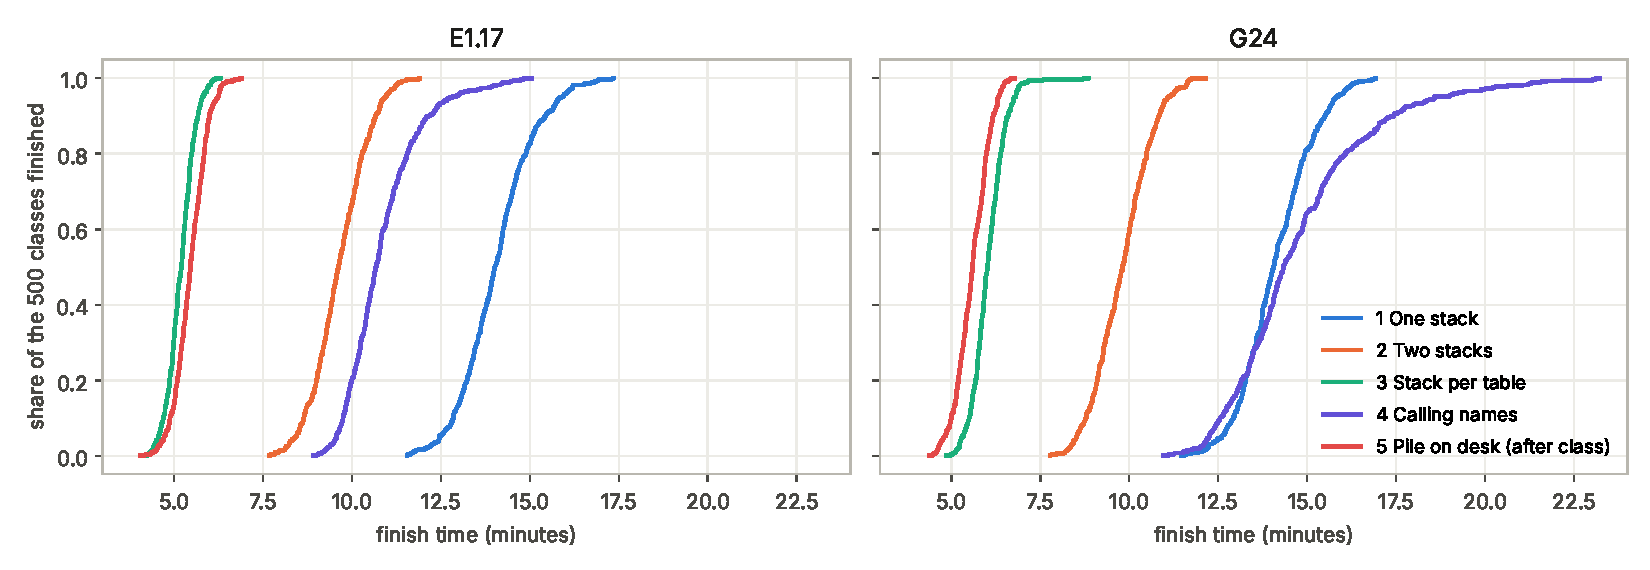
\includegraphics[width=\textwidth]{fig/ecdf.pdf}
\caption{Empirical cumulative distribution of finish times across the 500 classes. Curves further left are faster; steeper curves are more predictable.}\label{fig:ecdf}
\end{figure}

\subsection{Interpretation}
\begin{itemize}
  \item \textbf{One stack} is slow (about 14 minutes) but costs the lecturer only seconds and returns essentially every quiz (unclaimed 0.02 per class, consistent with $50q^2$).
  \item \textbf{Parallelism is what helps.} Two stacks save about 4.3 minutes; one stack per table saves 8--9 minutes. The price is lecturer time (up to 1.5 minutes in G24, where the lecturer walks the snake to place 10 stacks), much more disruption (2.5--3 times the student-minutes, 8--10 students busy at once instead of 1, and students getting up 26--31 times per class instead of 3--5) and slightly more unclaimed quizzes (Section~\ref{sec:certain}).
  \item \textbf{Calling names} is never better for this lecturer's goal: it costs all of its 11--14 minutes from teaching. It is the most variable method in G24, because of long walks and passing along benches.
  \item \textbf{The pile} is about as fast as one stack per table: 17\,s slower in E1.17 and 26\,s faster in G24. But it happens after class, and everyone stays behind for about 5.5 minutes.
\end{itemize}

\begin{figure}[htbp]\centering
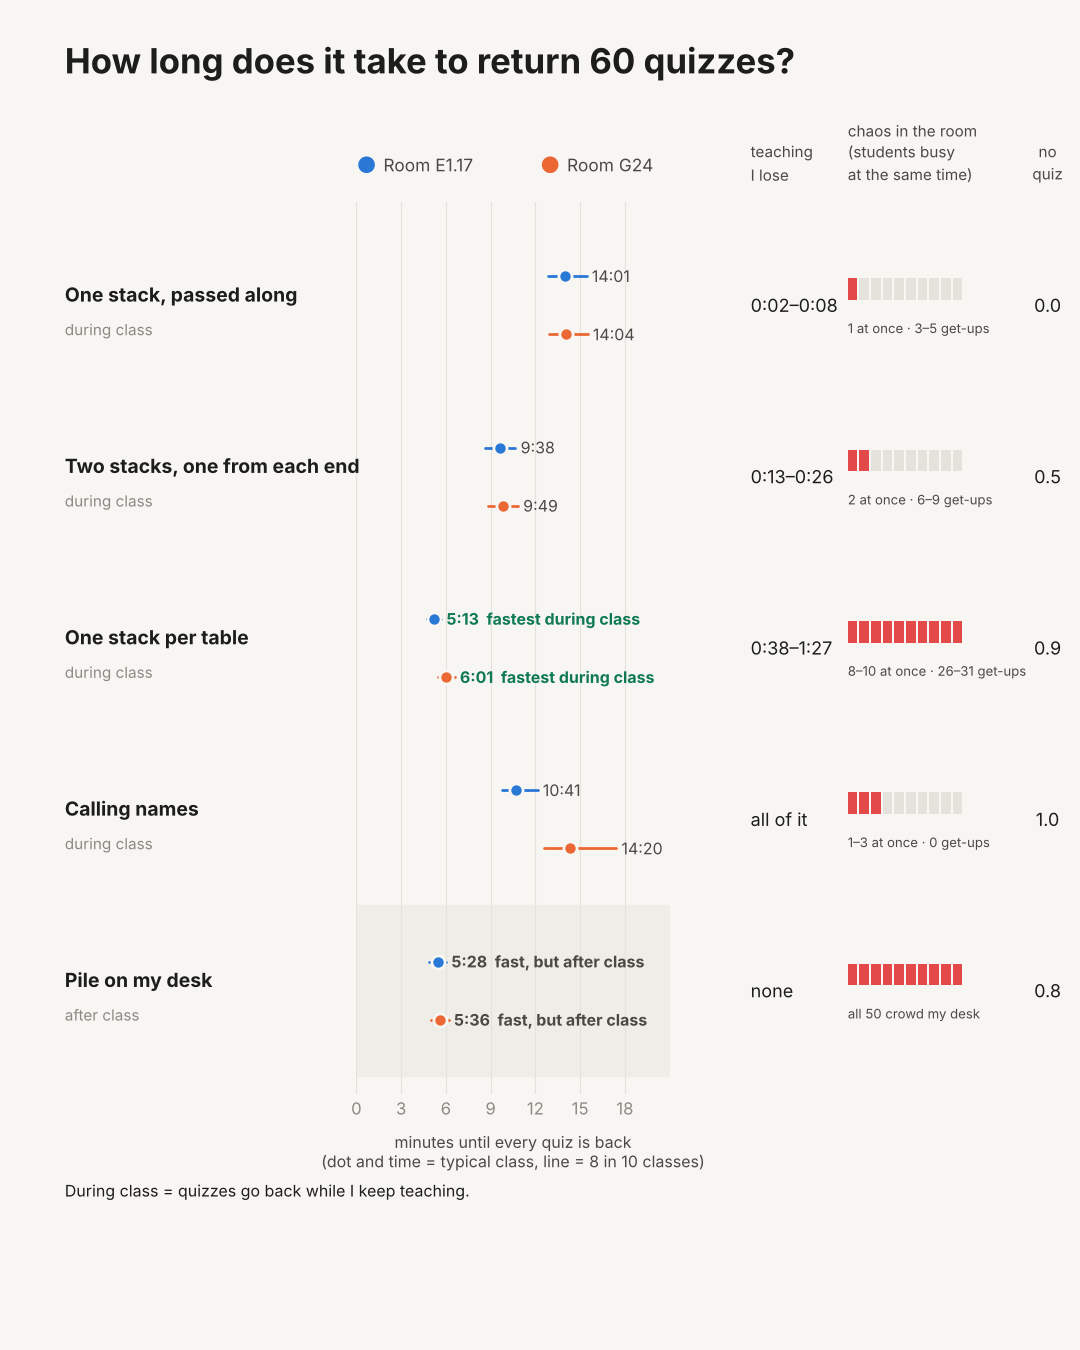
\includegraphics[width=0.62\textwidth]{fig/comparison.png}
\caption{Summary chart, as published.}
\end{figure}

%=====================================================================
\section{Sensitivity analysis}\label{sec:sensitivity}
Each assumed parameter was set to a low and a high value, one at a time, with everything else at its default (one-at-a-time design \cite{saltelli2008}).
Each setting uses the same 60 seeds (common random numbers). Entries are median finish times (mm:ss); the last column gives the in-class ranking (methods 1--4, fastest first). Method 5 is after class.

{\small\setlength{\tabcolsep}{4pt}
\begin{table}[htbp]\centering\footnotesize
\begin{tabular}{lrrrrrrl}
\toprule
Assumption (default) & Value & 1 & 2 & 3 & 4 & 5 & In-class ranking \\
\midrule
\textbf{Defaults} &  & 13:51 & 9:29 & 5:13 & 10:39 & 5:28 & 3<2<4<1 \\
b, seconds per sheet (0.6) & 0.3 & 9:10 & 6:42 & 4:21 & 10:39 & 4:12 & 3<2<1<4\,$\ast$ \\
 & 1.0 & 20:05 & 13:09 & 6:20 & 10:39 & 7:17 & 3<4<2<1\,$\ast$ \\
a, setup time (3 s) & 1.5 & 12:36 & 8:31 & 4:28 & 10:39 & 4:45 & 3<2<4<1 \\
 & 6.0 & 16:21 & 11:23 & 6:38 & 10:39 & 7:07 & 3<4<2<1\,$\ast$ \\
q, chance of missing your sheet (2\%) & 0.0 & 13:33 & 9:21 & 5:03 & 10:39 & 5:20 & 3<2<4<1 \\
 & 0.05 & 14:22 & 9:45 & 5:17 & 10:39 & 5:41 & 3<2<4<1 \\
reach for a seated hand-over (2.5 m) & 1.7 & 14:01 & 9:36 & 5:21 & 10:39 & 5:28 & 3<2<4<1 \\
 & 3.0 & 13:49 & 9:28 & 5:08 & 10:39 & 5:28 & 3<2<4<1 \\
hand-over time (2 s) & 1.0 & 13:02 & 8:39 & 4:27 & 9:54 & 5:28 & 3<2<4<1 \\
 & 4.0 & 15:39 & 11:17 & 6:52 & 12:17 & 5:28 & 3<2<4<1 \\
walking speed indoors ($\times$0.8) & 0.6 & 13:53 & 9:29 & 5:17 & 12:03 & 5:31 & 3<2<4<1 \\
 & 1.0 & 13:50 & 9:28 & 5:10 & 9:48 & 5:19 & 3<2<4<1 \\
chance a name needs repeating (30\%) & 0.0 & 13:51 & 9:29 & 5:13 & 9:45 & 5:28 & 3<2<4<1 \\
 & 0.6 & 13:51 & 9:29 & 5:13 & 11:48 & 5:28 & 3<2<4<1 \\
time to read a name (2 s) & 1.0 & 13:51 & 9:29 & 5:13 & 9:19 & 5:28 & 3<4<2<1\,$\ast$ \\
 & 4.0 & 13:51 & 9:29 & 5:13 & 13:25 & 5:28 & 3<2<4<1 \\
people at the pile at once (4) & 2 & 13:51 & 9:29 & 5:13 & 10:39 & 7:36 & 3<2<4<1 \\
 & 6 & 13:51 & 9:29 & 5:13 & 10:39 & 4:46 & 3<2<4<1 \\
patience before giving up (unlimited) & 120.0 & 13:51 & 9:29 & 5:13 & 10:39 & 3:38 & 3<2<4<1 \\
 & 600.0 & 13:51 & 9:29 & 5:13 & 10:39 & 5:26 & 3<2<4<1 \\
\bottomrule
\end{tabular}
\caption{Sensitivity, room E1.17. $\ast$ = in-class ranking differs from the default (3<2<4<1).}
\end{table}
\begin{table}[htbp]\centering\footnotesize
\begin{tabular}{lrrrrrrl}
\toprule
Assumption (default) & Value & 1 & 2 & 3 & 4 & 5 & In-class ranking \\
\midrule
\textbf{Defaults} &  & 13:56 & 9:47 & 6:01 & 14:23 & 5:40 & 3<2<1<4 \\
b, seconds per sheet (0.6) & 0.3 & 9:17 & 6:57 & 5:27 & 14:23 & 4:08 & 3<2<1<4 \\
 & 1.0 & 20:09 & 13:36 & 6:51 & 14:23 & 7:14 & 3<2<4<1\,$\ast$ \\
a, setup time (3 s) & 1.5 & 12:41 & 8:48 & 5:20 & 14:23 & 4:43 & 3<2<1<4 \\
 & 6.0 & 16:26 & 11:33 & 7:27 & 14:23 & 7:08 & 3<2<4<1\,$\ast$ \\
q, chance of missing your sheet (2\%) & 0.0 & 13:31 & 9:29 & 5:59 & 14:23 & 5:34 & 3<2<1<4 \\
 & 0.05 & 14:28 & 10:01 & 6:06 & 14:23 & 5:50 & 3<2<4<1\,$\ast$ \\
reach for a seated hand-over (2.5 m) & 1.7 & 14:07 & 9:56 & 6:20 & 14:23 & 5:40 & 3<2<1<4 \\
 & 3.0 & 13:54 & 9:43 & 5:53 & 14:23 & 5:40 & 3<2<1<4 \\
hand-over time (2 s) & 1.0 & 13:08 & 8:56 & 5:17 & 13:38 & 5:40 & 3<2<1<4 \\
 & 4.0 & 15:44 & 11:32 & 7:41 & 16:03 & 5:40 & 3<2<1<4 \\
walking speed indoors ($\times$0.8) & 0.6 & 14:00 & 9:53 & 6:37 & 16:58 & 5:37 & 3<2<1<4 \\
 & 1.0 & 13:54 & 9:43 & 5:43 & 12:50 & 5:34 & 3<2<4<1\,$\ast$ \\
chance a name needs repeating (30\%) & 0.0 & 13:56 & 9:47 & 6:01 & 13:32 & 5:40 & 3<2<4<1\,$\ast$ \\
 & 0.6 & 13:56 & 9:47 & 6:01 & 15:37 & 5:40 & 3<2<1<4 \\
time to read a name (2 s) & 1.0 & 13:56 & 9:47 & 6:01 & 13:01 & 5:40 & 3<2<4<1\,$\ast$ \\
 & 4.0 & 13:56 & 9:47 & 6:01 & 17:14 & 5:40 & 3<2<1<4 \\
people at the pile at once (4) & 2 & 13:56 & 9:47 & 6:01 & 14:23 & 7:39 & 3<2<1<4 \\
 & 6 & 13:56 & 9:47 & 6:01 & 14:23 & 4:59 & 3<2<1<4 \\
patience before giving up (unlimited) & 120.0 & 13:56 & 9:47 & 6:01 & 14:23 & 3:46 & 3<2<1<4 \\
 & 600.0 & 13:56 & 9:47 & 6:01 & 14:23 & 5:35 & 3<2<1<4 \\
\bottomrule
\end{tabular}
\caption{Sensitivity, room G24. $\ast$ = in-class ranking differs from the default (3<2<1<4).}
\end{table}
}

\paragraph{Summary.} Across 40 settings (both rooms), the in-class ranking changed in 10. In every setting, one stack per table (3) was the fastest in-class method, and two stacks (2) beat one stack (1). Every change in ranking involved only the position of calling names (4), which competes closely with one stack in G24 (14:20 vs 14:04 at the defaults) and with two stacks when search is slow. Search speed $b$ has by far the largest effect on the stack methods (one stack: about 9--20 minutes over $b=0.3$--$1.0$\,s), which is why measuring it is the first priority.


%=====================================================================
\section{Limitations}
\begin{enumerate}
  \item \textbf{Room dimensions are estimated} from sketches (Section~\ref{sec:space}). Measured plans will replace them.
  \item \textbf{Behavioural parameters} ($a$, $b$, $q$, hand-over and slide times, calling-names timings, pile access and swap time) are assumptions, and are tested in Section~\ref{sec:sensitivity}. The single most influential, $b$, can be calibrated by timing one stack's lap in class: with Section~\ref{sec:verification}, total time $\approx 50(a+2) + 912.5\,b + {}$walking.
  \item \textbf{Seating is uniform at random;} real students cluster with friends and favour certain rows.
  \item \textbf{Social behaviour is omitted:} chatting, helping, glancing at friends' grades.
  \item \textbf{The passing route is idealised;} real classes will deviate.
  \item \textbf{Simplified crowd model:} the pile uses a deterministic floor field, not the full stochastic model with dynamic field, and chunk contents are not updated during a search.
  \item \textbf{Timing only:} disruption is reported as student-minutes, times students get up and the peak number busy at once; it is not converted into lost learning, and noise or attention drift in students not involved is not modelled.
\end{enumerate}

%=====================================================================
\section{Questions you may be asked}
\begin{description}[style=nextline]
\item[Why a grid model and not a continuous one such as the social-force model?]
The social-force model \cite{helbing1995} resolves body-to-body forces, which matter for dense, fast crowds. Here movement is short, slow and mostly single-file, and the dominant cost is searching, not walking. A CA with 0.4\,m cells is the standard, much cheaper approximation \cite{burstedde2001,kirchner2002}.
\item[Why $\Delta t = 0.1$\,s?]
At 1.07\,m/s a person crosses a 0.4\,m cell in about 0.37\,s, so each step resolves a fraction of a cell. Hand-over and search times (seconds) are resolved to 0.1\,s.
\item[Why is the position of your sheet uniform? Isn't that assumed?]
It is not assumed: it is a property of a uniform shuffle (Proposition 1), and the code produces it by actually shuffling (Figure~\ref{fig:position} and the $\chi^2$ test in Section~\ref{sec:verification}). Proposition 2 shows it stays uniform as sheets are removed.
\item[Why linear in the number of sheets?]
Flicking through a stack is inspecting items one at a time until the target is found: serial self-terminating search, whose reaction time is linear in the number inspected \cite{treisman1980,wolfe1998}.
\item[Why log-normal for $b$?]
Human response times are positive and right-skewed \cite{luce1986}. A log-normal is the simplest two-parameter law with those properties. Its mean is fixed at 0.6\,s, so $\E[T]$ is unaffected by the choice of shape.
\item[Are $b$ and $K$ independent?]
Yes. $b$ is a property of the student and $K$ of the shuffle, drawn from separate random numbers. Hence $\E[bK]=\E[b]\E[K]$.
\item[Why does splitting into stacks not reduce reading?]
Section~\ref{sec:multi}: $\E[C] = (R+1)/2$ for any number of equal stacks. The time saving of multi-stack methods is purely from parallel searching.
\item[Why only misses and no false matches?]
Taking someone else's quiz would require misreading a different name as one's own. We assume this is negligible compared with overlooking one's own sheet.
\item[Is 500 runs enough?]
The standard errors of the medians are 3--7\,s (bootstrap intervals in Table~\ref{tab:results}), and the paired differences between methods are tens to hundreds of seconds with intervals excluding zero, except where reported as ties.
\item[Why the median and the 10th--90th percentiles?]
The distributions are skewed (Figure~\ref{fig:ecdf}), and the median and percentiles are robust to that. Means and standard deviations are in the raw data.
\item[Why common random numbers?]
They make comparisons paired. The variance of a difference between methods is $\Var(X)+\Var(Y)-2\operatorname{Cov}(X,Y)$, and the shared seating and shuffle make the covariance positive \cite{law2015}.
\item[How would you validate the model?]
Time one real stack lap in each room and compare with the predicted distribution (13--15.6 minutes for one stack). Then refit $b$, the main free parameter, from the observed total.
\item[How do I reproduce everything?]
\texttt{python run\_experiments.py} (results), \texttt{python run\_sensitivity.py} (Section~\ref{sec:sensitivity}), \texttt{python tests/test\_search\_math.py} and \texttt{python tests/test\_sanity.py} (verification), \texttt{python make\_videos.py} and \texttt{python make\_chart.py} (figures). The software used was Python 3.13, NumPy 2.5, Matplotlib 3.11, PyYAML 6.0 and FFmpeg 6.1.
\end{description}

%=====================================================================
\appendix
\section{All parameters}
\begin{table}[htbp]\centering\small
\begin{tabularx}{\textwidth}{lXl}
\toprule
Parameter & Value & Basis \\
\midrule
Quizzes / present / absent & 60 / 50 / 10 & lecturer \\
Grid cell; time step & 0.4\,m; 0.1\,s & \cite{burstedde2001} \\
Free walking speed & $\mathcal N(1.34, 0.26^2)$ m/s, clipped $[0.7, 2.0]$ & \cite{weidmann1993} \\
Indoor factor & 0.8 & assumption \\
Setup time $a$ & 3.0\,s & assumption \\
Time per sheet $b$ & log-normal, mean 0.6\,s, CV 0.3 & assumption (agreed); shape \cite{luce1986} \\
Miss probability $q$; passes when certain & 0.02; 2 & assumption \\
Hand-over; seated reach & 2.0\,s; 2.5\,m & assumption \\
Slide past empty seats & 0.6\,s per metre beyond reach & assumption \\
Drop leftovers on desk & 1.0\,s & assumption \\
Calling: read; repeat prob.\ (max) & 2.0\,s; 0.3 (2) & assumption \\
Calling: absent silence; not recognised & 4.0\,s; 0.02 & assumption \\
Calling: hand up; lecturer reach; bench pass & 1.5\,s; 1.0\,m; 1.5\,s per seat & assumption \\
Pile: packing up; access spots; max at pile & $U(0,20)$\,s; 8; 4 & assumption \\
Pile: chunk swap; patience & 3.0\,s; effectively unlimited & assumption; lecturer's observation \\
Crowd: counter-flow swap; sideways shuffle & 0.3; 0.2 per step & modelling device \\
Re-plan after blocked & 2.0\,s & modelling device \\
Runs per method and room; seeds & 500; 0--499 & -- \\
\bottomrule
\end{tabularx}
\end{table}

\begin{thebibliography}{99}\small
\bibitem{burstedde2001} C.~Burstedde, K.~Klauck, A.~Schadschneider and J.~Zittartz (2001). Simulation of pedestrian dynamics using a two-dimensional cellular automaton. \emph{Physica A}, 295, 507--525.
\bibitem{kirchner2002} A.~Kirchner and A.~Schadschneider (2002). Simulation of evacuation processes using a bionics-inspired cellular automaton model for pedestrian dynamics. \emph{Physica A}, 312, 260--276.
\bibitem{weidmann1993} U.~Weidmann (1993). \emph{Transporttechnik der Fussg\"anger}. Schriftenreihe des IVT Nr.~90, ETH Z\"urich.
\bibitem{helbing1995} D.~Helbing and P.~Moln\'ar (1995). Social force model for pedestrian dynamics. \emph{Physical Review E}, 51, 4282--4286.
\bibitem{dijkstra1959} E.~W.~Dijkstra (1959). A note on two problems in connexion with graphs. \emph{Numerische Mathematik}, 1, 269--271.
\bibitem{treisman1980} A.~M.~Treisman and G.~Gelade (1980). A feature-integration theory of attention. \emph{Cognitive Psychology}, 12, 97--136.
\bibitem{wolfe1998} J.~M.~Wolfe (1998). What can 1 million trials tell us about visual search? \emph{Psychological Science}, 9(1), 33--39.
\bibitem{luce1986} R.~D.~Luce (1986). \emph{Response Times: Their Role in Inferring Elementary Mental Organization}. Oxford University Press.
\bibitem{brysbaert2019} M.~Brysbaert (2019). How many words do we read per minute? A review and meta-analysis of reading rate. \emph{Journal of Memory and Language}, 109, 104047.
\bibitem{kleinrock1975} L.~Kleinrock (1975). \emph{Queueing Systems, Volume 1: Theory}. Wiley.
\bibitem{law2015} A.~M.~Law (2015). \emph{Simulation Modeling and Analysis}, 5th ed. McGraw-Hill.
\bibitem{efron1993} B.~Efron and R.~J.~Tibshirani (1993). \emph{An Introduction to the Bootstrap}. Chapman \& Hall.
\bibitem{saltelli2008} A.~Saltelli et al.\ (2008). \emph{Global Sensitivity Analysis: The Primer}. Wiley.
\bibitem{oneill2014} M.~E.~O'Neill (2014). PCG: A family of simple fast space-efficient statistically good algorithms for random number generation. Technical report HMC-CS-2014-0905, Harvey Mudd College.
\bibitem{steffen2008} J.~H.~Steffen (2008). Optimal boarding method for airline passengers. \emph{Journal of Air Transport Management}, 14(3), 146--150.
\end{thebibliography}

\end{document}
